\documentclass{article}
\usepackage[utf8]{inputenc}
\usepackage{amsmath}
\usepackage{graphicx}
\graphicspath{ {./images/} }

\title{Tarea 02 de Circuitos Lineales I}
\author{Gabriel Gamboa Vargas}
\date{Octubre 2021}

\begin{document}

\maketitle

\section{Ejercicio 1}
Se aplica la LCK a cada nodo usando los nombres de tensiones de nodo que el ejercicio incluye.

\begin{equation} 
    2A + \frac{v3-v1}{6\Omega} = \frac{v1}{2\Omega}
\end{equation}

\begin{equation}
    2A + \frac{v2-v4}{10\Omega} + \frac{v2}{5\Omega} = \frac{v3-v2}{2\Omega}
\end{equation}
    
\begin{equation}
    1A = \frac{v3-v2}{2\Omega} + \frac{v3-v1}{6\Omega} + \frac{v3-v4}{5\Omega}
\end{equation}

\begin{equation}
    \frac{v3-v4}{5\Omega} + \frac{v2-v4}{10\Omega} = \frac{v4}{5\Omega}
\end{equation}

\begin{equation}
    \frac{v7-v5}{4\Omega} = \frac{v5}{1\Omega} + 2A
\end{equation}
    
\begin{equation}
    2A + \frac{v7-v6}{2\Omega} = \frac{v6-v8}{4\Omega} + \frac{v6}{4\Omega}
\end{equation}

\begin{equation}
    6A = \frac{v7-v6}{2\Omega} + \frac{v7-v5}{4\Omega} + \frac{v7-v8}{10\Omega}
\end{equation}

\begin{equation}
    \frac{v7-v8}{10\Omega} + \frac{v6-v8}{4\Omega} = \frac{v8}{1\Omega}
\end{equation}

Se tienen 8 ecuaciones lineales con 8 incógnitas, se puede construir una matriz 8x8 para encontrar sus soluciones. 
La primer columna se asocia con v1, la segunda con v2 y se mantendrá ese patrón con las demás. \\ \\ \\
$
\begin{pmatrix}
    2/3 & 0 & -1/6 & 0 & 0 & 0 & 0 & 0\\
    0 & -4/5 & 1/2 & 1/10 & 0 & 0 & 0 & 0\\
    -1/6 & -1/2 & 13/15 & -1/5 & 0 & 0 & 0 & 0\\
    0 & 1/10 & 1/5 & -1/2 & 0 & 0 & 0 & 0\\ 
    0 & 0 & 0 & 0 & -5/4 & 0 & 1/4 & 0\\ 
    0 & 0 & 0 & 0 & 0 & 1 & -1/2 & -1/4\\
    0 & 0 & 0 & 0 & -1/4 & -1/2 & 17/20 & -1/10\\ 
    0 & 0 & 0 & 0 & 0 & 1/4 & 1/10 & -27/20\\ 
\end{pmatrix}
$$\begin{bmatrix}
    v1 \\
    v2 \\
    v3 \\
    v4 \\
    v5 \\
    v6\\
    v7\\
    v8
\end{bmatrix}
$ = $\begin{bmatrix}
    2 \\
    2 \\
    1 \\
    0 \\
    2 \\
    2\\
    6\\
    0
\end{bmatrix}
$ \\ \\ \\
f1 = 3/2 F1 \\ \\
$
\begin{pmatrix}
    1 & 0 & -1/4 & 0 & 0 & 0 & 0 & 0\\
    0 & -4/5 & 1/2 & 1/10 & 0 & 0 & 0 & 0\\
    -1/6 & -1/2 & 13/15 & -1/5 & 0 & 0 & 0 & 0\\
    0 & 1/10 & 1/5 & -1/2 & 0 & 0 & 0 & 0\\ 
    0 & 0 & 0 & 0 & -5/4 & 0 & 1/4 & 0\\ 
    0 & 0 & 0 & 0 & 0 & 1 & -1/2 & -1/4\\
    0 & 0 & 0 & 0 & -1/4 & -1/2 & 17/20 & -1/10\\ 
    0 & 0 & 0 & 0 & 0 & 1/4 & 1/10 & -27/20\\ 
\end{pmatrix}
$$\begin{bmatrix}
    v1 \\
    v2 \\
    v3 \\
    v4 \\
    v5 \\
    v6\\
    v7\\
    v8
\end{bmatrix}
$ = $\begin{bmatrix}
    3 \\
    2 \\
    1 \\
    0 \\
    2 \\
    2\\
    6\\
    0
\end{bmatrix}
$ \\ \\ \\
F3 = 1/6 F1 +F3 \\ \\
$
\begin{pmatrix}
    1 & 0 & -1/4 & 0 & 0 & 0 & 0 & 0\\
    0 & -4/5 & 1/2 & 1/10 & 0 & 0 & 0 & 0\\
    0 & -1/2 & 33/40 & -1/5 & 0 & 0 & 0 & 0\\
    0 & 1/10 & 1/5 & -1/2 & 0 & 0 & 0 & 0\\ 
    0 & 0 & 0 & 0 & -5/4 & 0 & 1/4 & 0\\ 
    0 & 0 & 0 & 0 & 0 & 1 & -1/2 & -1/4\\
    0 & 0 & 0 & 0 & -1/4 & -1/2 & 17/20 & -1/10\\ 
    0 & 0 & 0 & 0 & 0 & 1/4 & 1/10 & -27/20\\ 
\end{pmatrix}
$$\begin{bmatrix}
    v1 \\
    v2 \\
    v3 \\
    v4 \\
    v5 \\
    v6\\
    v7\\
    v8
\end{bmatrix}
$ = $\begin{bmatrix}
    3 \\
    2 \\
    3/2 \\
    0 \\
    2 \\
    2\\
    6\\
    0
\end{bmatrix}
$ \\ \\ \\
F2 = -5/4 F2 \\ \\ 
$
\begin{pmatrix}
    1 & 0 & -1/4 & 0 & 0 & 0 & 0 & 0\\
    0 & 1 & -5/8 & -1/8 & 0 & 0 & 0 & 0\\
    0 & -1/2 & 33/40 & -1/5 & 0 & 0 & 0 & 0\\
    0 & 1/10 & 1/5 & -1/2 & 0 & 0 & 0 & 0\\ 
    0 & 0 & 0 & 0 & -5/4 & 0 & 1/4 & 0\\ 
    0 & 0 & 0 & 0 & 0 & 1 & -1/2 & -1/4\\
    0 & 0 & 0 & 0 & -1/4 & -1/2 & 17/20 & -1/10\\ 
    0 & 0 & 0 & 0 & 0 & 1/4 & 1/10 & -27/20\\ 
\end{pmatrix}
$$\begin{bmatrix}
    v1 \\
    v2 \\
    v3 \\
    v4 \\
    v5 \\
    v6\\
    v7\\
    v8
\end{bmatrix}
$ = $\begin{bmatrix}
    3 \\
    -5/2 \\
    3/2 \\
    0 \\
    2 \\
    2\\
    6\\
    0
\end{bmatrix}
$\\ \\ 
F3 = 1/2 F2 + F3 \\
F4 = -1/10 F2 + F4 \\
$
\begin{pmatrix}
    1 & 0 & -1/4 & 0 & 0 & 0 & 0 & 0\\
    0 & 1 & -5/8 & -1/8 & 0 & 0 & 0 & 0\\
    0 & 0 & 41/80 & -21/80 & 0 & 0 & 0 & 0\\
    0 & 0 & 21/80 & -39/80 & 0 & 0 & 0 & 0\\ 
    0 & 0 & 0 & 0 & -5/4 & 0 & 1/4 & 0\\ 
    0 & 0 & 0 & 0 & 0 & 1 & -1/2 & -1/4\\
    0 & 0 & 0 & 0 & -1/4 & -1/2 & 17/20 & -1/10\\ 
    0 & 0 & 0 & 0 & 0 & 1/4 & 1/10 & -27/20\\ 
\end{pmatrix}
$$\begin{bmatrix}
    v1 \\
    v2 \\
    v3 \\
    v4 \\
    v5 \\
    v6\\
    v7\\
    v8
\end{bmatrix}
$ = $\begin{bmatrix}
    3 \\
    -5/2 \\
    1/4 \\
    1/4 \\
    2 \\
    2\\
    6\\
    0
\end{bmatrix}
$\\ \\ 
F3 = 80/41 F3 \\ \\
$
\begin{pmatrix}
    1 & 0 & -1/4 & 0 & 0 & 0 & 0 & 0\\
    0 & 1 & -5/8 & -1/8 & 0 & 0 & 0 & 0\\
    0 & 0 & 1 & -21/41 & 0 & 0 & 0 & 0\\
    0 & 0 & 21/80 & -39/80 & 0 & 0 & 0 & 0\\ 
    0 & 0 & 0 & 0 & -5/4 & 0 & 1/4 & 0\\ 
    0 & 0 & 0 & 0 & 0 & 1 & -1/2 & -1/4\\
    0 & 0 & 0 & 0 & -1/4 & -1/2 & 17/20 & -1/10\\ 
    0 & 0 & 0 & 0 & 0 & 1/4 & 1/10 & -27/20\\ 
\end{pmatrix}
$$\begin{bmatrix}
    v1 \\
    v2 \\
    v3 \\
    v4 \\
    v5 \\
    v6\\
    v7\\
    v8
\end{bmatrix}
$ = $\begin{bmatrix}
    3 \\
    -5/2 \\
    20/41 \\
    1/4 \\
    2 \\
    2\\
    6\\
    0
\end{bmatrix}
$\\ \\ 
F4 = -21/80 F3 + F4 \\ \\
$
\begin{pmatrix}
    1 & 0 & -1/4 & 0 & 0 & 0 & 0 & 0\\
    0 & 1 & -5/8 & -1/8 & 0 & 0 & 0 & 0\\
    0 & 0 & 1 & -21/41 & 0 & 0 & 0 & 0\\
    0 & 0 & 0 & -579/1640 & 0 & 0 & 0 & 0\\ 
    0 & 0 & 0 & 0 & -5/4 & 0 & 1/4 & 0\\ 
    0 & 0 & 0 & 0 & 0 & 1 & -1/2 & -1/4\\
    0 & 0 & 0 & 0 & -1/4 & -1/2 & 17/20 & -1/10\\ 
    0 & 0 & 0 & 0 & 0 & 1/4 & 1/10 & -27/20\\ 
\end{pmatrix}
$$\begin{bmatrix}
    v1 \\
    v2 \\
    v3 \\
    v4 \\
    v5 \\
    v6\\
    v7\\
    v8
\end{bmatrix}
$ = $\begin{bmatrix}
    3 \\
    -5/2 \\
    20/41 \\
    5/41 \\
    2 \\
    2\\
    6\\
    0
\end{bmatrix}
$\\ \\ 
F4 = -1640/579 F4 \\ \\ 
$
\begin{pmatrix}
    1 & 0 & -1/4 & 0 & 0 & 0 & 0 & 0\\
    0 & 1 & -5/8 & -1/8 & 0 & 0 & 0 & 0\\
    0 & 0 & 1 & -21/41 & 0 & 0 & 0 & 0\\
    0 & 0 & 0 & 1 & 0 & 0 & 0 & 0\\ 
    0 & 0 & 0 & 0 & -5/4 & 0 & 1/4 & 0\\ 
    0 & 0 & 0 & 0 & 0 & 1 & -1/2 & -1/4\\
    0 & 0 & 0 & 0 & -1/4 & -1/2 & 17/20 & -1/10\\ 
    0 & 0 & 0 & 0 & 0 & 1/4 & 1/10 & -27/20\\ 
\end{pmatrix}
$$\begin{bmatrix}
    v1 \\
    v2 \\
    v3 \\
    v4 \\
    v5 \\
    v6\\
    v7\\
    v8
\end{bmatrix}
$ = $\begin{bmatrix}
    3 \\
    -5/2 \\
    20/41 \\
    -200/579 \\
    2 \\
    2\\
    6\\
    0
\end{bmatrix}
$\\ \\ 
F5 = -4/5 F5 \\ \\ 
$
\begin{pmatrix}
    1 & 0 & -1/4 & 0 & 0 & 0 & 0 & 0\\
    0 & 1 & -5/8 & -1/8 & 0 & 0 & 0 & 0\\
    0 & 0 & 1 & -21/41 & 0 & 0 & 0 & 0\\
    0 & 0 & 0 & 1 & 0 & 0 & 0 & 0\\ 
    0 & 0 & 0 & 0 & 1 & 0 & -1/5 & 0\\ 
    0 & 0 & 0 & 0 & 0 & 1 & -1/2 & -1/4\\
    0 & 0 & 0 & 0 & -1/4 & -1/2 & 17/20 & -1/10\\ 
    0 & 0 & 0 & 0 & 0 & 1/4 & 1/10 & -27/20\\ 
\end{pmatrix}
$$\begin{bmatrix}
    v1 \\
    v2 \\
    v3 \\
    v4 \\
    v5 \\
    v6\\
    v7\\
    v8
\end{bmatrix}
$ = $\begin{bmatrix}
    3 \\
    -5/2 \\
    20/41 \\ \\
    -200/579 \\
    -8/5 \\
    2\\
    6\\
    0
\end{bmatrix}
$\\ \\ 
F7 = 1/4 F5 + F7 \\ \\ 
$
\begin{pmatrix}
    1 & 0 & -1/4 & 0 & 0 & 0 & 0 & 0\\
    0 & 1 & -5/8 & -1/8 & 0 & 0 & 0 & 0\\
    0 & 0 & 1 & -21/41 & 0 & 0 & 0 & 0\\
    0 & 0 & 0 & 1 & 0 & 0 & 0 & 0\\ 
    0 & 0 & 0 & 0 & 1 & 0 & -1/5 & 0\\ 
    0 & 0 & 0 & 0 & 0 & 1 & -1/2 & -1/4\\
    0 & 0 & 0 & 0 & 0 & -1/2 & 4/5 & -1/10\\ 
    0 & 0 & 0 & 0 & 0 & 1/4 & 1/10 & -27/20\\ 
\end{pmatrix}
$$\begin{bmatrix}
    v1 \\
    v2 \\
    v3 \\
    v4 \\
    v5 \\
    v6\\
    v7\\
    v8
\end{bmatrix}
$ = $\begin{bmatrix}
    3 \\
    -5/2 \\
    20/41 \\
    -200/579 \\
    -8/5 \\
    2\\
    28/5\\
    0
\end{bmatrix}
$\\ \\ 
F7 = 1/2 F6 + F7\\
F8 = -1/4 F6 + F8\\ \\
$
\begin{pmatrix}
    1 & 0 & -1/4 & 0 & 0 & 0 & 0 & 0\\
    0 & 1 & -5/8 & -1/8 & 0 & 0 & 0 & 0\\
    0 & 0 & 1 & -21/41 & 0 & 0 & 0 & 0\\
    0 & 0 & 0 & 1 & 0 & 0 & 0 & 0\\ 
    0 & 0 & 0 & 0 & 1 & 0 & -1/5 & 0\\ 
    0 & 0 & 0 & 0 & 0 & 1 & -1/2 & -1/4\\
    0 & 0 & 0 & 0 & 0 & 0 & 11/20 & -9/40\\ 
    0 & 0 & 0 & 0 & 0 & 0 & 9/40 & -103/80\\ 
\end{pmatrix}
$$\begin{bmatrix}
    v1 \\
    v2 \\
    v3 \\
    v4 \\
    v5 \\
    v6\\
    v7\\
    v8
\end{bmatrix}
$ = $\begin{bmatrix}
    3 \\
    -5/2 \\
    20/41 \\
    -200/579 \\
    -8/5 \\
    2\\
    33/5\\
    -1/2
\end{bmatrix}
$\\ \\ 
F7 = 20/11 F7 \\ \\ 
$
\begin{pmatrix}
    1 & 0 & -1/4 & 0 & 0 & 0 & 0 & 0\\
    0 & 1 & -5/8 & -1/8 & 0 & 0 & 0 & 0\\
    0 & 0 & 1 & -21/41 & 0 & 0 & 0 & 0\\
    0 & 0 & 0 & 1 & 0 & 0 & 0 & 0\\ 
    0 & 0 & 0 & 0 & 1 & 0 & -1/5 & 0\\ 
    0 & 0 & 0 & 0 & 0 & 1 & -1/2 & -1/4\\
    0 & 0 & 0 & 0 & 0 & 0 & 1 & -9/22\\ 
    0 & 0 & 0 & 0 & 0 & 0 & 9/40 & -103/80\\ 
\end{pmatrix}
$$\begin{bmatrix}
    v1 \\
    v2 \\
    v3 \\
    v4 \\
    v5 \\
    v6\\
    v7\\
    v8
\end{bmatrix}
$ = $\begin{bmatrix}
    3 \\
    -5/2 \\
    20/41 \\
    -200/579 \\
    -8/5 \\
    2\\
    12\\
    -1/2
\end{bmatrix}
$\\ \\ 
F8 = -9/40 F7 + F8 \\ \\
$
\begin{pmatrix}
    1 & 0 & -1/4 & 0 & 0 & 0 & 0 & 0\\
    0 & 1 & -5/8 & -1/8 & 0 & 0 & 0 & 0\\
    0 & 0 & 1 & -21/41 & 0 & 0 & 0 & 0\\
    0 & 0 & 0 & 1 & 0 & 0 & 0 & 0\\ 
    0 & 0 & 0 & 0 & 1 & 0 & -1/5 & 0\\ 
    0 & 0 & 0 & 0 & 0 & 1 & -1/2 & -1/4\\
    0 & 0 & 0 & 0 & 0 & 0 & 1 & -9/22\\ 
    0 & 0 & 0 & 0 & 0 & 0 & 0 & -263/220\\ 
\end{pmatrix}
$$\begin{bmatrix}
    v1 \\
    v2 \\
    v3 \\
    v4 \\
    v5 \\
    v6\\
    v7\\
    v8
\end{bmatrix}
$ = $\begin{bmatrix}
    3 \\
    -5/2 \\
    20/41 \\ \\
    -200/579 \\
    -8/5 \\
    2\\
    12\\
    -16/5
\end{bmatrix}
$\\ \\ 
F8 = -220/263 F8 \\ \\ 
$
\begin{pmatrix}
    1 & 0 & -1/4 & 0 & 0 & 0 & 0 & 0\\
    0 & 1 & -5/8 & -1/8 & 0 & 0 & 0 & 0\\
    0 & 0 & 1 & -21/41 & 0 & 0 & 0 & 0\\
    0 & 0 & 0 & 1 & 0 & 0 & 0 & 0\\ 
    0 & 0 & 0 & 0 & 1 & 0 & -1/5 & 0\\ 
    0 & 0 & 0 & 0 & 0 & 1 & -1/2 & -1/4\\
    0 & 0 & 0 & 0 & 0 & 0 & 1 & -9/22\\ 
    0 & 0 & 0 & 0 & 0 & 0 & 0 & 1\\ 
\end{pmatrix}
$$\begin{bmatrix}
    v1 \\
    v2 \\
    v3 \\
    v4 \\
    v5 \\
    v6\\
    v7\\
    v8
\end{bmatrix}
$ = $\begin{bmatrix}
    3 \\
    -5/2 \\
    20/41 \\ \\
    -200/579 \\
    -8/5 \\
    2\\
    12\\
    704/263
\end{bmatrix}
$\\ \\ 
F6 = 1/4 F8 + F6 \\
F7 = 9/22 F8 + F7 \\ \\ 
$
\begin{pmatrix}
    1 & 0 & -1/4 & 0 & 0 & 0 & 0 & 0\\
    0 & 1 & -5/8 & -1/8 & 0 & 0 & 0 & 0\\
    0 & 0 & 1 & -21/41 & 0 & 0 & 0 & 0\\
    0 & 0 & 0 & 1 & 0 & 0 & 0 & 0\\ 
    0 & 0 & 0 & 0 & 1 & 0 & -1/5 & 0\\ 
    0 & 0 & 0 & 0 & 0 & 1 & -1/2 & 0\\
    0 & 0 & 0 & 0 & 0 & 0 & 1 & 0\\ 
    0 & 0 & 0 & 0 & 0 & 0 & 0 & 1\\ 
\end{pmatrix}
$$\begin{bmatrix}
    v1 \\
    v2 \\
    v3 \\
    v4 \\
    v5 \\
    v6\\
    v7\\
    v8
\end{bmatrix}
$ = $\begin{bmatrix}
    3 \\
    -5/2 \\
    20/41 \\
    -200/579 \\
    -8/5 \\
    702/263\\
    3444/263\\
    704/263
\end{bmatrix}
$\\ \\ 
F6 = 1/2 F7 + F6 \\ \\ 
$
\begin{pmatrix}
    1 & 0 & -1/4 & 0 & 0 & 0 & 0 & 0\\
    0 & 1 & -5/8 & -1/8 & 0 & 0 & 0 & 0\\
    0 & 0 & 1 & -21/41 & 0 & 0 & 0 & 0\\
    0 & 0 & 0 & 1 & 0 & 0 & 0 & 0\\ 
    0 & 0 & 0 & 0 & 1 & 0 & -1/5 & 0\\ 
    0 & 0 & 0 & 0 & 0 & 1 & 0 & 0\\
    0 & 0 & 0 & 0 & 0 & 0 & 1 & 0\\ 
    0 & 0 & 0 & 0 & 0 & 0 & 0 & 1\\ 
\end{pmatrix}
$$\begin{bmatrix}
    v1 \\
    v2 \\
    v3 \\
    v4 \\
    v5 \\
    v6\\
    v7\\
    v8
\end{bmatrix}
$ = $\begin{bmatrix}
    3 \\
    -5/2 \\
    20/41 \\
    -200/579 \\
    -8/5 \\
    2424/263\\
    3444/263\\
    704/263
\end{bmatrix}
$\\ \\ 
F5 = 1/5 F7 + F5 \\ \\
$
\begin{pmatrix}
    1 & 0 & -1/4 & 0 & 0 & 0 & 0 & 0\\
    0 & 1 & -5/8 & -1/8 & 0 & 0 & 0 & 0\\
    0 & 0 & 1 & -21/41 & 0 & 0 & 0 & 0\\
    0 & 0 & 0 & 1 & 0 & 0 & 0 & 0\\ 
    0 & 0 & 0 & 0 & 1 & 0 & 0 & 0\\ 
    0 & 0 & 0 & 0 & 0 & 1 & 0 & 0\\
    0 & 0 & 0 & 0 & 0 & 0 & 1 & 0\\ 
    0 & 0 & 0 & 0 & 0 & 0 & 0 & 1\\ 
\end{pmatrix}
$$\begin{bmatrix}
    v1 \\
    v2 \\
    v3 \\
    v4 \\
    v5 \\
    v6\\
    v7\\
    v8
\end{bmatrix}
$ = $\begin{bmatrix}
    3 \\
    -5/2 \\
    20/41 \\
    -200/579 \\
    268/263 \\
    2424/263\\
    3444/263\\
    704/263
\end{bmatrix}
$\\ \\ 
F3 = 21/41 F4 + F3\\ \\
$
\begin{pmatrix}
    1 & 0 & -1/4 & 0 & 0 & 0 & 0 & 0\\
    0 & 1 & -5/8 & -1/8 & 0 & 0 & 0 & 0\\
    0 & 0 & 1 & 0 & 0 & 0 & 0 & 0\\
    0 & 0 & 0 & 1 & 0 & 0 & 0 & 0\\ 
    0 & 0 & 0 & 0 & 1 & 0 & 0 & 0\\ 
    0 & 0 & 0 & 0 & 0 & 1 & 0 & 0\\
    0 & 0 & 0 & 0 & 0 & 0 & 1 & 0\\ 
    0 & 0 & 0 & 0 & 0 & 0 & 0 & 1\\ 
\end{pmatrix}
$$\begin{bmatrix}
    v1 \\
    v2 \\
    v3 \\
    v4 \\
    v5 \\
    v6\\
    v7\\
    v8
\end{bmatrix}
$ = $\begin{bmatrix}
    3 \\
    -5/2 \\
    60/193 \\
    -200/579 \\
    268/263 \\
    2424/263\\
    3444/263\\
    704/263
\end{bmatrix}
$\\ \\ 
F2 = 1/8 F4 + F2 \\ \\
$
\begin{pmatrix}
    1 & 0 & -1/4 & 0 & 0 & 0 & 0 & 0\\
    0 & 1 & -5/8 & 0 & 0 & 0 & 0 & 0\\
    0 & 0 & 1 & 0 & 0 & 0 & 0 & 0\\
    0 & 0 & 0 & 1 & 0 & 0 & 0 & 0\\ 
    0 & 0 & 0 & 0 & 1 & 0 & 0 & 0\\ 
    0 & 0 & 0 & 0 & 0 & 1 & 0 & 0\\
    0 & 0 & 0 & 0 & 0 & 0 & 1 & 0\\ 
    0 & 0 & 0 & 0 & 0 & 0 & 0 & 1\\ 
\end{pmatrix}
$$\begin{bmatrix}
    v1 \\
    v2 \\
    v3 \\
    v4 \\
    v5 \\
    v6\\
    v7\\
    v8
\end{bmatrix}
$ = $\begin{bmatrix}
    3 \\
    -2945/1158 \\
    60/193 \\
    -200/579 \\
    268/263 \\
    2424/263\\
    3444/263\\
    704/263
\end{bmatrix}
$\\ \\ 
F2 = 5/8 F3 + F2 \\ \\
$
\begin{pmatrix}
    1 & 0 & -1/4 & 0 & 0 & 0 & 0 & 0\\
    0 & 1 & 0 & 0 & 0 & 0 & 0 & 0\\
    0 & 0 & 1 & 0 & 0 & 0 & 0 & 0\\
    0 & 0 & 0 & 1 & 0 & 0 & 0 & 0\\ 
    0 & 0 & 0 & 0 & 1 & 0 & 0 & 0\\ 
    0 & 0 & 0 & 0 & 0 & 1 & 0 & 0\\
    0 & 0 & 0 & 0 & 0 & 0 & 1 & 0\\ 
    0 & 0 & 0 & 0 & 0 & 0 & 0 & 1\\ 
\end{pmatrix}
$$\begin{bmatrix}
    v1 \\
    v2 \\
    v3 \\
    v4 \\
    v5 \\
    v6\\
    v7\\
    v8
\end{bmatrix}
$ = $\begin{bmatrix}
    3 \\
    -1360/579 \\
    60/193 \\
    -200/579 \\
    268/263 \\
    2424/263\\
    3444/263\\
    704/263
\end{bmatrix}
$\\ \\ 
F1 = 1/4 F3 + F1 \\ \\
$
\begin{pmatrix}
    1 & 0 & 0 & 0 & 0 & 0 & 0 & 0\\
    0 & 1 & 0 & 0 & 0 & 0 & 0 & 0\\
    0 & 0 & 1 & 0 & 0 & 0 & 0 & 0\\
    0 & 0 & 0 & 1 & 0 & 0 & 0 & 0\\ 
    0 & 0 & 0 & 0 & 1 & 0 & 0 & 0\\ 
    0 & 0 & 0 & 0 & 0 & 1 & 0 & 0\\
    0 & 0 & 0 & 0 & 0 & 0 & 1 & 0\\ 
    0 & 0 & 0 & 0 & 0 & 0 & 0 & 1\\ 
\end{pmatrix}
$$\begin{bmatrix}
    v1 \\
    v2 \\
    v3 \\
    v4 \\
    v5 \\
    v6\\
    v7\\
    v8
\end{bmatrix}
$ = $\begin{bmatrix}
    594/193 \\
    -1360/579 \\
    60/193 \\
    -200/579 \\
    268/263 \\
    2424/263\\
    3444/263\\
    704/263
\end{bmatrix}
$\\ \\ \\ \\
v1 = 594/193 V = 3.07772V\\
v2 = -1360/579 V = -2.34888V\\
v3 = 60/193 V = 0.310881V\\
v4 = -200/579 V = -0.345423V\\
v5 = 268/263 V = 1.01901V\\
v6 = 2424/263 V = 9.21673V\\
v7 = 3444/263 V = 13.0951V\\
v8 = 704/263 V =  2.67681V\\ \\ \\
\section{Ejercicio 2}
Parte A: \\ \\
Se aplica la LCK a cada nodo ya nombrado en el ejercicio.

\begin{equation}
    2A = v1-v2 + 2v1 + 4(v1-v3) + 1.5K = 7v1 - v2 -4v3 + 1.5K 
\end{equation}

\begin{equation}
    v1-v2 = v2-v3 + 4v2
\end{equation}

\begin{equation}
    v2-v3 + 4A + 1.5K + 4(v1-v3) =  2v3
\end{equation}

Como $4v2 = 1.5 \Longrightarrow -v2 = -3/8 \land 6v2 = 9/4 \land v2 = 3/8$

\begin{equation}
    2A = 7v1 - 3/8 -4v3 + 1.5K 
\end{equation}

\begin{equation}
    v1 = -v3 + 9/4
\end{equation}

\begin{equation}
    3/8-v3 + 4A + 1.5K + 4(v1-v3) =  2v3
\end{equation}
Sustituyendo (13) en (12): \\ \\
$v3 = -(2A - 123/8 -1.5K)/11 = 107/88  + \frac{3K}{22}$ \\ \\
Resolviendo para v1: \\ \\
$v1 = 91/88  - \frac{3K}{22}$ \\ \\
Note que a medida que v3 se hace más grande v1 se hace más pequeño al mismo ritmo, lo que permite que la potencia del circuito se mantenga constante sin necesidad de que v2 cambie, por lo tanto cualquier valor de K da un circuito funcional sin cambiar v2.\\ \\
Parte B:\\ \\ 
$K = 8$\\ \\
$v1 = 91/88 - \frac{12}{11} = \frac{-5}{88}V$\\ \\
$v3 = 107/88 + \frac{12}{11} = \frac{203}{88}V$\\
\section{Ejercicio 3}
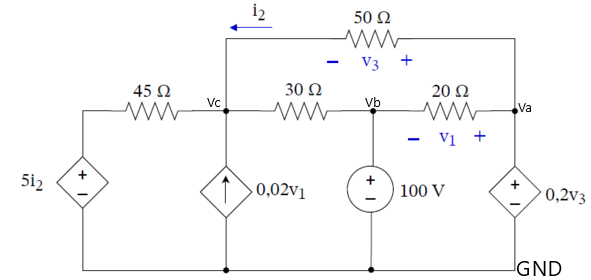
\includegraphics[]{images/ejercicio3_2.PNG} \\ \\ \\
\begin{equation}
    Va = 0.2V3
\end{equation}
\begin{equation}
    Vb = 100V
\end{equation}
\begin{equation}
    Va - Vc = V3
\end{equation}
Aplicando LTK en GND, Va y Vb y despejando
\begin{equation}
    500V+5V1=V3 
\end{equation}
Se aplica LCK en el nodo Vc: \\ \\
\begin{equation}
    \frac{500V+5V1}{50\Omega} + \frac{100V-Vc}{30\Omega} + 0,02V1= \frac{Vc}{45\Omega} -\frac{500V + 5V1}{450\Omega} 
\end{equation}
Note: \\
\begin{equation}
    Vc = -4/5 V3 \Longrightarrow Vc = -400V -4V1
\end{equation}
Sustituyendo (20) en (19):\\ \\
v1 = -103.7735849V\\ \\
Resolviendo (18) para V3:\\ \\
V3 = -18.8679245V
\end{document}
